%% 
%% Copyright 2007-2024 Elsevier Ltd
%% 
%% This file is part of the 'Elsarticle Bundle'.
%% ---------------------------------------------
%% 
%% It may be distributed under the conditions of the LaTeX Project Public
%% License, either version 1.3 of this license or (at your option) any
%% later version.  The latest version of this license is in
%%    http://www.latex-project.org/lppl.txt
%% and version 1.3 or later is part of all distributions of LaTeX
%% version 1999/12/01 or later.
%% 
%% The list of all files belonging to the 'Elsarticle Bundle' is
%% given in the file `manifest.txt'.
%% 
%% Template article for Elsevier's document class `elsarticle'
%% with numbered style bibliographic references
%% SP 2008/03/01
%% $Id: elsarticle-template-num.tex 249 2024-04-06 10:51:24Z rishi $
%%
%%\documentclass[preprint,12pt]{elsarticle}

% Final Manuscript Preparation Notes.  Adam Stephen 2024/11/10
%
% Specifically trying to solve a problem with Reference Generation.
%
% From Elsevier Help, the following points were useful.
%
% 1. In case of issues - email elsarticle@stmdocs.in
% 2. There is a beginner course online.
% 3. 

\newif\ifpreprint
\preprinttrue
%\preprintfalse
%

\ifpreprint
\documentclass[preprint]{elsarticle}
\else
\documentclass[5p]{elsarticle}
\fi

%% Use the option review to obtain double line spacing
%% \documentclass[authoryear,preprint,review,12pt]{elsarticle}

%% Use the options 1p,twocolumn; 3p; 3p,twocolumn; 5p; or 5p,twocolumn
%% for a journal layout:
%% \documentclass[final,1p,times]{elsarticle}
%% \documentclass[final,1p,times,twocolumn]{elsarticle}
%% \documentclass[final,3p,times]{elsarticle}
%% \documentclass[final,3p,times,twocolumn]{elsarticle}
%% \documentclass[final,5p,times]{elsarticle}
%% \documentclass[final,5p,times,twocolumn]{elsarticle}

%% For including figures, graphicx.sty has been loaded in
%% elsarticle.cls. If you prefer to use the old commands
%% please give \usepackage{epsfig}

%% The amssymb package provides various useful mathematical symbols
\usepackage{amssymb}
%% The amsmath package provides various useful equation environments.
\usepackage{amsmath}
%% The amsthm package provides extended theorem environments
%% \usepackage{amsthm}

%% The lineno packages adds line numbers. Start line numbering with
%% \begin{linenumbers}, end it with \end{linenumbers}. Or switch it on
%% for the whole article with \linenumbers.
%% \usepackage{lineno}

% Own Packages
%\usepackage{float}

\journal{Fusion Engineering and Design}

\begin{document}

\begin{frontmatter}

%% Title, authors and addresses

%% use the tnoteref command within \title for footnotes;
%% use the tnotetext command for theassociated footnote;
%% use the fnref command within \author or \affiliation for footnotes;
%% use the fntext command for theassociated footnote;
%% use the corref command within \author for corresponding author footnotes;
%% use the cortext command for theassociated footnote;
%% use the ead command for the email address,
%% and the form \ead[url] for the home page:
%% \title{Title\tnoteref{label1}}
%% \tnotetext[label1]{}
%% \author{Name\corref{cor1}\fnref{label2}}
%% \ead{email address}
%% \ead[url]{home page}
%% \fntext[label2]{}
%% \cortext[cor1]{}
%% \affiliation{organization={},
%%             addressline={},
%%             city={},
%%             postcode={},
%%             state={},
%%             country={}}
%% \fntext[label3]{}

\title{JET Plasma Control System Upgrade using MARTe2}

%% use optional labels to link authors explicitly to addresses:
%% \author[label1,label2]{}
%% \affiliation[label1]{organization={},
%%             addressline={},
%%             city={},
%%             postcode={},
%%             state={},
%%             country={}}
%%
%% \affiliation[label2]{organization={},
%%             addressline={},
%%             city={},
%%             postcode={},
%%             state={},
%%             country={}}

	\author[UKAEA]{A.V.~Stephen} %% Author name
	%\author[UKAEA]{A.V.~Stephen\corref{cor1}} %% Author name
	\ead{adam.stephen@ukaea.uk}
%% \author{Name\corref{cor1}\fnref{label2}}
%% \ead{email address}
\author[UKAEA]{A.~Goodyear}
\author[UKAEA]{D.~Valcarcel}
\author[UKAEA]{J.~Waterhouse}
\author[UKAEA]{E.~Jones}
\author[UKAEA]{P.A.~McCullen}
\author[UKAEA]{C.~Boswell}
\author[UKAEA]{N.~Petrella}
\author[UKAEA]{P.~Fox}
\author[UKAEA]{M.~Lennholm}
\author[UKAEA]{M.~Wheatley}
\author[UKAEA]{H.~Baker}
\author[UKAEA]{A.~Parrott}
\author[UKAEA]{K.~Purahoo}
\author[UKAEA]{M.~Anderton}
\author[UKAEA]{C.~Stuart}
\author[UKAEA]{D.~Collishaw-Shepman}
\author[UKAEA]{R.~Padden}

%% Author affiliation
%\affiliation{organization={Computing Division, United Kingdom Atomic Energy Authority},%Department and Organization
	\affiliation[UKAEA]{organization={United Kingdom Atomic Energy Authority},%Organization
            addressline={Culham Campus}, 
            city={Abingdon},
            postcode={OX14 3DB}, 
            state={Oxfordshire},
            country={United Kingdom}}

%% Abstract
\begin{abstract}
%% Text of abstract

JET real-time plasma control has been delivered with a heterogeneous collection of control systems linked by a dedicated low-jitter, low-latency network. To provide a high degree of flexibility in tuning plasma control algorithms to experimental requirements, the Real-Time Central Controller (RTCC) has been available since 1997. RTCC provides a sandboxed execution environment where experimental algorithms can be deployed with a rapid development workflow. New control laws can be developed by operators during the course of an experimental session. The potential impact of a defect in algorithms evolved without full lifecycle quality assurance can be bounded by clipping feedback control requests at the actuator managers. The likelihood of such defects is reduced in the first place by constraining the algorithms to be composed from reusable blocks and trusted real-time signals. Although this system operated successfully for a long time, limitations in compute capacity of the legacy hardware on which the application was deployed constrained algorithm development.

Motivated by the need to provide physics operators with a more performant system, an upgrade project was carried out to port the RTCC application to a modern high performance PC platform. The architecture selected was to use the MARTe2 framework. Development was able to reuse existing MARTe2 data sources to connect the application to the JET environment using the ITER SDN protocol. RTCC blocks were converted to MARTe2 functions. Python tooling was created to automatically convert previously deployed RTCC algorithms to MARTe2 configuration form.

This paper describes the techniques used to demonstrate system correctness prior to deployment in the JET operating environment. This was particularly important given that it was deployed around the time of the DT campaigns. It explains how the system was used to demonstrate some novel control methods which delivered useful experiments in the final JET campaigns. It also outlines how the JET legacy data combined with this MARTe2 application can offer future value, even in the absence of the JET machine itself.
\end{abstract}

%%Graphical abstract
%% TODO: This is recommended
%\begin{graphicalabstract}
%\includegraphics{grabs}
%\end{graphicalabstract}

%% TODO: This is recommended
%%Research highlights
%%\begin{highlights}
%\item Research highlight 1
%\item Research highlight 2
%\end{highlights}

%% Keywords
\begin{keyword}
%% keywords here, in the form: keyword \sep keyword
real-time \sep control \sep MARTe2 \sep JET \sep QA

%% PACS codes here, in the form: \PACS code \sep code

%% MSC codes here, in the form: \MSC code \sep code
%% or \MSC[2008] code \sep code (2000 is the default)

\end{keyword}

\end{frontmatter}

%% Add \usepackage{lineno} before \begin{document} and uncomment 
%% following line to enable line numbers
%% \linenumbers

%% main text
%%

%% Use \section commands to start a section
\section{Introduction}
\label{sec:intro}
%% Labels are used to cross-reference an item using \ref command.

%\subsection{Background}

Plasma Control Systems\footnote{PCS - Plasma Control System} are large and complex.
There are variations in approach, but most fusion projects distinguish between
the disciplines of physics design and real-time system implementation.

Physics design is informed by, but usually separate from, first principles 
high-fidelity simulation. It works with macroscopic plasma quantities
and involves reduced order models with sufficient simplification to admit
practical use in a real-time environment.  This discipline combines
physics understanding of the main plasma and machine processes, along
with engineering control theory. Development typically uses modelling 
environments and may make use of experimental or synthetic data.

Real-time system implementation is tasked with converting the physics design
into a robust and resilient deterministic control system.  It must reproduce
the expected behaviour from the design system, in the real-world environment.
One challenge is to prove that the algorithm outcomes do not diverge from
the predicted path when running on different hardware, implemented in different
languages and frameworks. The performance of the code (in all possible paths) 
must be shown to be compatible with the dynamics time scales.  Delay is an enemy of 
control, time jitter effectively injects noise into a process.
The code must be free of race conditions, memory or other resource leaks
and defects.  If generated by tools, then those tools must be verified.
If generated by manual coding, adequate unit and integration tests must
be performed. 

In both cases, it is necessary to provide tooling and processes which support
evolution of the design, and the implementation.  This means tracking versions,
configuration, input data sets experienced by the codes, and the results and
verification of the correctness of these.  The lifecycle must also define
for how to iterate, when to migrate new features from design to implementation,
and how to commission and deploy.

Finally, management of off-normal events (often termed {\em exceptions}) 
must be addressed.  From the design point of view, exceptions include both
failure of the design to achieve control of the process dynamics (error of method)
as well as failure of equipment which prevents control (error of measurement or actuator).
Mitigations defined in the design must be implemented in real-time.  In addition
the real-time system must be able to degrade gracefully in the event of internal
exceptions (hardware faults or system corruption).

One of the design strategies for the JET plasma control system was to include
a flexible real-time central controller (RTCC). This was capable of 
supporting physics design activity in an inherently real-time environment
with integrated support for managing off-normal events.
This enabled very rapid prototyping of new control
algorithms during the course of JET experimental sessions
without triggering an iteration of software development.

This paper describes why it was necessary to upgrade JET RTCC as part of the
final JET operations campaigns.  It describes how the JET design principles
and system architectures reduced the risk and cost of this project to a 
level that made if feasible.  It describes the outcomes of the project, 
including the additional benefits that the work leaves for the future
exploitation of the JET data.


%The former abstracts higher level descriptions of the plasma control processes
%from the physics perspective. Thus dealing with magnetic, kinetic, MHD and error field
%control as well as wall conditioning, disruption and runaway electron control.
%Real-time system implementation must then map the control tasks into robust, resilient,
%deterministic control software. The implementation must deal with practical real-world
%constraints. These include signal processing to compute the required algorithm
%inputs, management of target control references throughout the shot, and provision 
%of exceptional handling strategies to resolve off-normal conditions (whether in the plasma,
%or in the sensor and actuator subsystems).

% TODO\cite
% https://www.sciencedirect.com/science/article/abs/pii/S0920379614000647
% Physics of the conceptual design of the ITER plasma control system 
%
%
% NO IT DOESN'T : IT DESCRIBES ONE UPGRADE WHICH TACKLED BOTH-ish

%This paper concentrates on the second challenge, of real-time plasma control system implementation.

%The order of the paper is $\ldots$ % TODO



% RENAME Materials and Methods, but that is the spirit
\section{Infrastructure and Architecture}

\subsection{JET PCS Infrastructure}
\label{l_infrastructure}

The JET PCS infrastructure was distributed and
heterogeneous\footnote{JET has entered decommissioning, and although the PCS systems still exist, they no longer operate.}.  
It was divided into around 80 subsystems spanning measurement, control, and protection functions.
This separation was required partly for organisational reasons: to divide the responsibility, and the work.
It was also beneficial to achieve sufficient decoupling to permit evolution without excessive risk.

The variability in technologies in implementation arose partly from differences in
optimal design choices and constraints across the project.  It was also enforced
as the project lifetime extended and as generations of software and hardware
evolved through industry cycles.

Where collections of subsystems were required to work collectively, real-time data was
shared as required. As one example, magnetics sensor data was acquired by the KC1D
diagnostic, and provided to the plasma shape and position controller.  During early
phases of the project, these real-time links were dedicated point to point connections.
The infrastructure became more fully connected with the introduction of a comprehensive
real-time data network.  This was initially implemented using Asynchronous Transfer Mode (ATM)
telecomms technology (effective, but highly bespoke). A later upgrade extended the
real-time network using standard ethernet equipment, and adopting the ITER Synchronous Databus
Network (SDN\cite{boncagniSynchronousDatabusNetwork2008}) protocol.


\subsection{JET PCS Architecture}
\label{l_architecture}

The JET PCS architecture is shown in figure~\ref{fig:pcs}. 
It comprises four main groups: measurements, local feedback, global feedback and actuators.
The arrows indicate information flows, including pre-configured parameter values, and
real-time data.  Some of the core functions operate mostly within the inner local feedback
loop.  This includes the main magnetic, heating and fuelling loops.  More sophisticated
control, and protection, are provided through the real-time central controller (RTCC) 
and auxiliary real-time signal server (RTSS).

Each of the individual systems may be implemented using a variety of technology.
The unifying aspects of the architecture are a standard real-time data exchange
protocol\cite{feltonRealtimeMeasurementControl2005b}, and a common parameter management system (Level-1\cite{vanderbekenLevelSoftwareJET1989}).

\ifpreprint
\begin{figure}[!p]
\else
\begin{figure}[ht!]
\fi

\centering

\ifpreprint
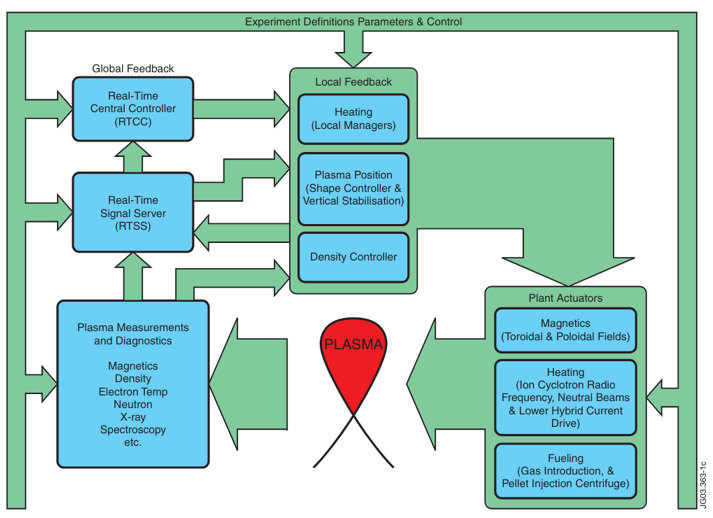
\includegraphics[width=1.0\textwidth]{JG_Felton.PNG}
\else
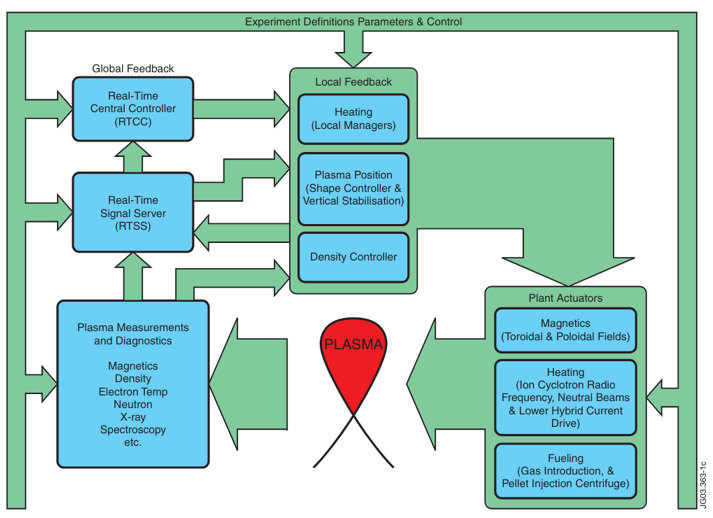
\includegraphics[width=0.5\textwidth]{JG_Felton.PNG}
\fi
\caption{The JET Plasma Control System (PCS) architecture from \cite{feltonRealtimeMeasurementControl2005b}.}
\label{fig:pcs}
\end{figure}

\subsection{JET Real-Time Central Controller}
\label{s_rtcc}

The function of the standard local control systems was to establish 
common plasma operating states (scenarios), mostly based on 
pre-calculated feed-forward references (with feedback control to stabilise
around particular operating points).  As such, these control systems
had a stable development lifecycle, with modifications and enhancements
generally being implemented during long shutdown periods.

To provide more advanced control, of plasma parameters for which the
relationship between direct measurement and fixed actuator response, 
it was necessary to add a more flexible and dynamic controller.
This real-time central controller (RTCC) provided a library of
reusable calculation blocks.  Using a custom editor, the physics
operator was permitted to design a control algorithm as a 
sequential graph (or {\em network}) of up to 200 blocks.
Up to four concurrent RTCC networks could be executed.

Figure~\ref{fig:tf} shows the documentation for one of these calculation
blocks (a first order transfer function). Each block received a variable
number of analogue inputs (continuously varying signals) as well as
one digital input. Blocks to express logical combinations, as well as
signal transformation were provided.  
The RTCC networks could therefore encompass 
control flow as well as signal processing.

Provision was made for all of the
usual mathematical operators, as well as for higher level functions such
as waveform generation, and PID control.  One limitation was that
only scalar valued signals could be treated.  Vector oriented control
schemes were possible, but had to be expressed as sets of scalar 
expressions.

\ifpreprint
\begin{figure}[p]
\else
\begin{figure}[ht!]
\fi
\centering
\ifpreprint
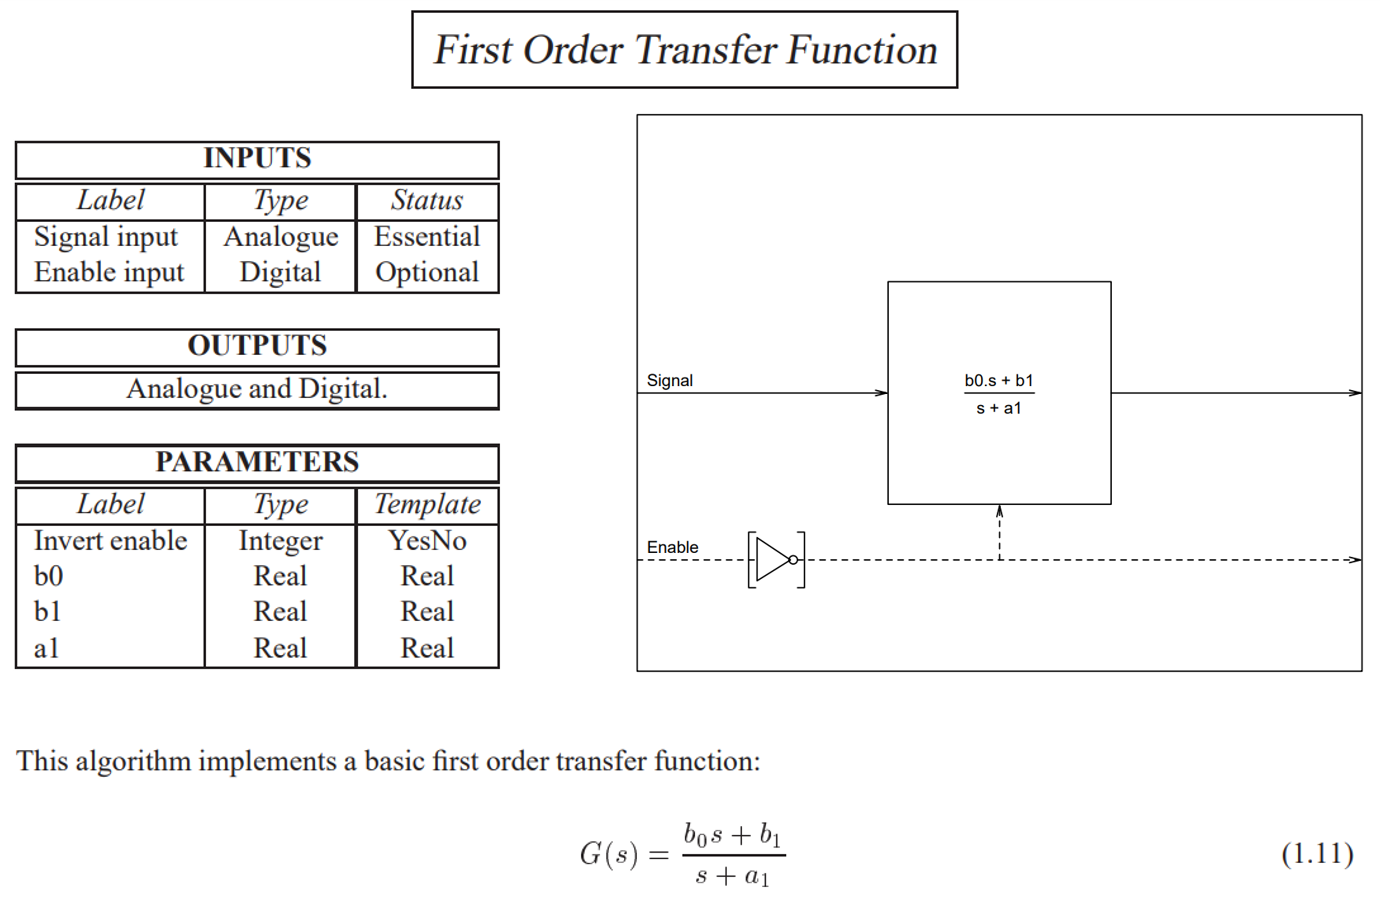
\includegraphics[width=1.0\textwidth]{RTCC_TF1_BLOCK.PNG}
\else
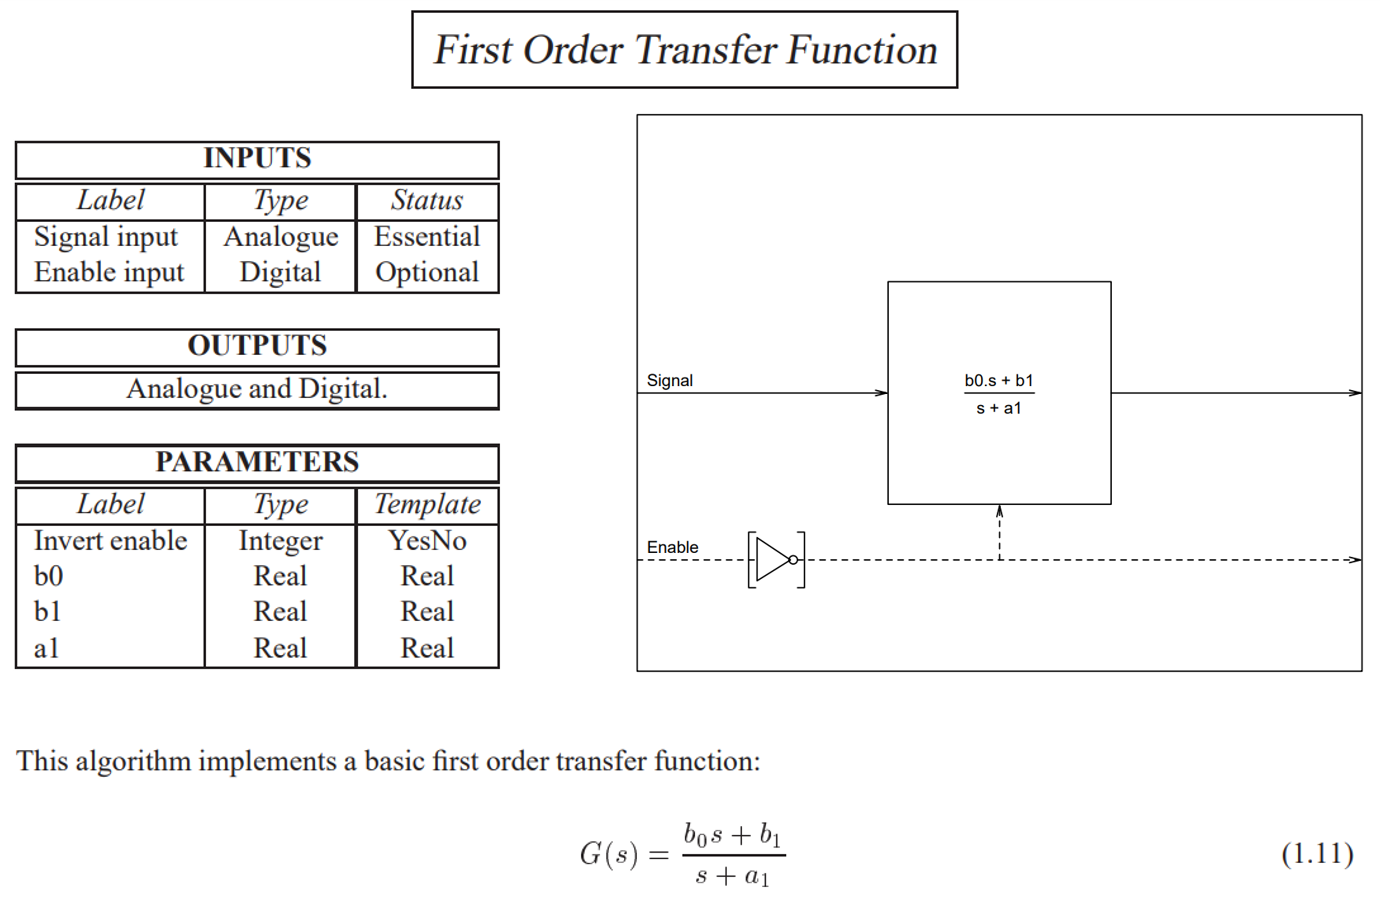
\includegraphics[width=0.5\textwidth]{RTCC_TF1_BLOCK.PNG}
\fi
\caption{The first order transfer function block. One of approximately 40 reusable components
	available for physics operators to design control schemes on-the-fly in RTCC.}
\label{fig:tf}
\end{figure}

Using this toolkit, a specialist operator---the Plasma Duty Officer (PDO)
would take instruction from the Session Leader (SL) as to the required
control schemes needed to support an experimental session.
The PDO team built an extensive library of RTCC networks.
Typical responsibilities for the PDO could be to modify the
networks to probe and tune gains, to replace diagnostic
signals by alternatives or to develop entirely new schemes.

The software tools to support the role were sufficient, but
required training and had some idiosynchrasies and limitations.
Proposals to improve the applications were put forward, but
ease of use was not seen as a sufficiently high priority to
allocate resources.  Figure~\ref{fig:editor} shows the tabular
graph editor. Each row on the left instantiates one of the 
blocks, and the output is assigned to the identifier on the right.
While a supporting viewer which could render the defined network
as a graph was available, the graphical view did not support
editing.

\ifpreprint
\begin{figure}[p]
\else
\begin{figure}[ht!]
\fi
\centering
\ifpreprint
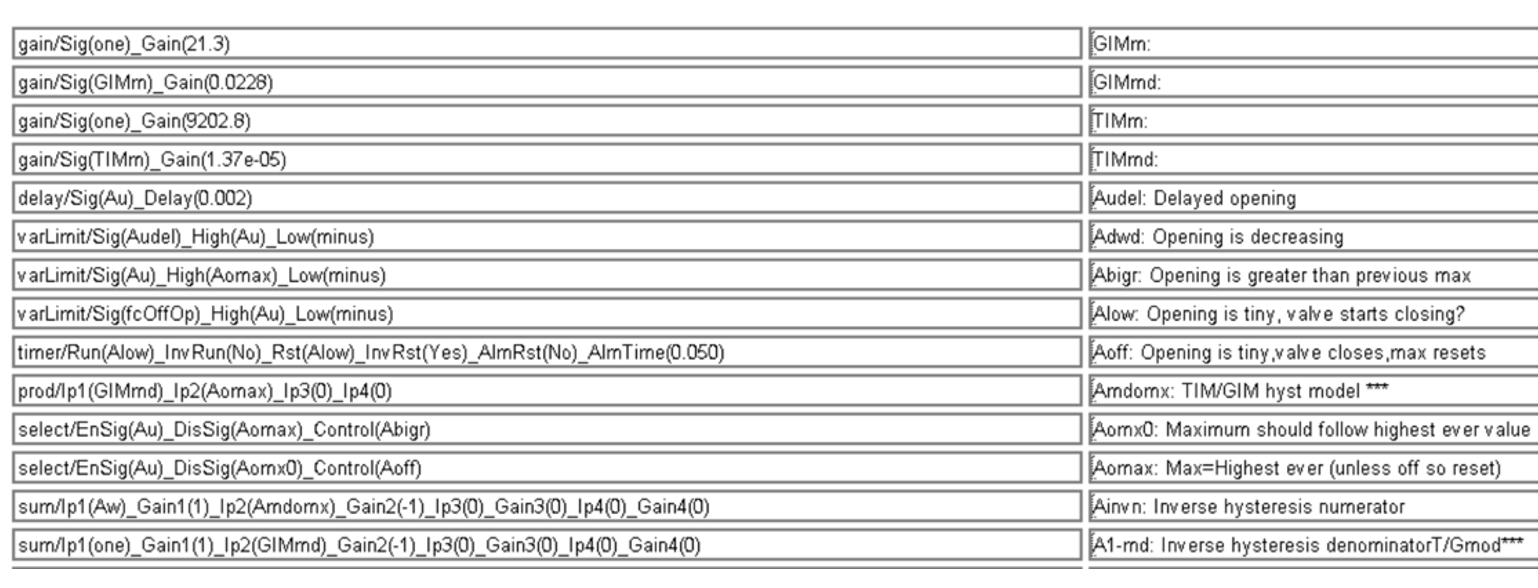
\includegraphics[width=1.0\textwidth]{L1RTCC.PNG}
\else
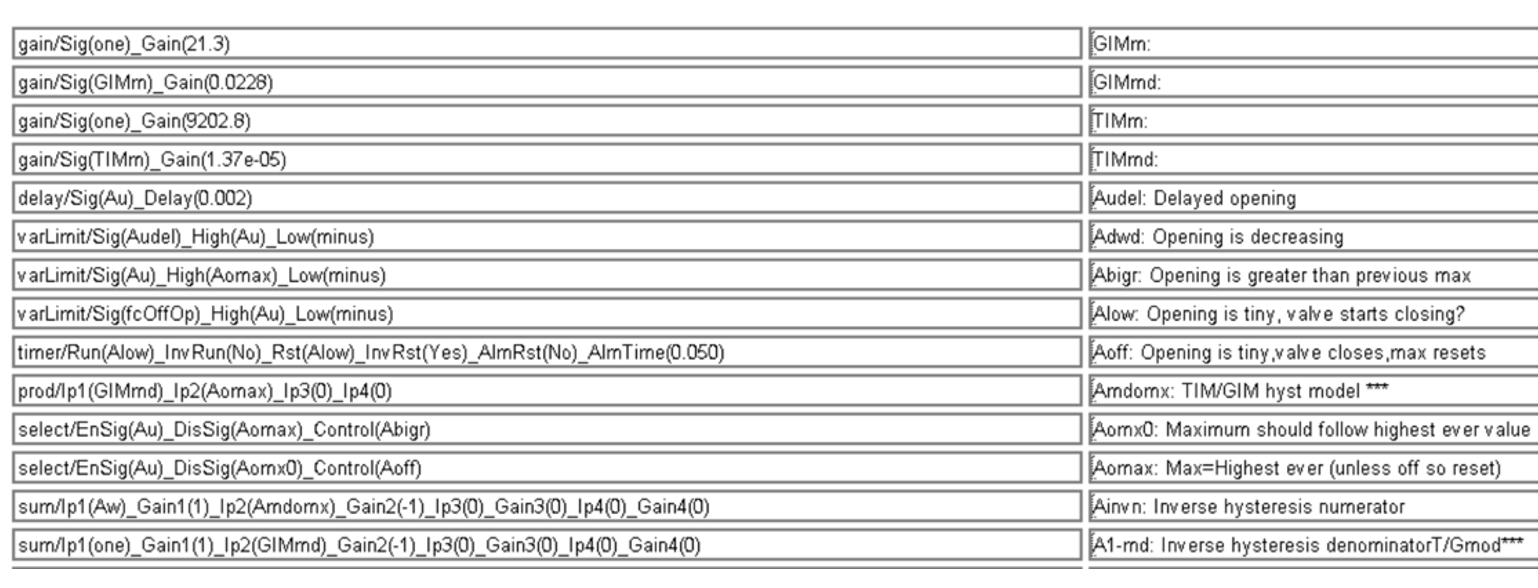
\includegraphics[width=0.5\textwidth]{L1RTCC.PNG}
\fi
\caption{The tabular RTCC network editor, implemented in JET Level-1 software.}\label{fig:editor}
\end{figure}


%Termed the {\em real-time central controller (RTCC)} this system was
%part of a suite of general real-time services targeting advanced
%real-time control research.  The RTCC system was an application 
%capable of receiving a very wide (and variable) set of input signals
%aggregated and managed by a companion system, the {\em real-time signal server (RTSS)}.
%
%The architecture of this RTCC application was the common pattern of
%a real-time execution engine configurable with a graph of signal
%processing blocks.  The library of blocks supported signal ingress,
%filtering and validation to achieve estimates of plasma parameter
%state.  Entities to implement control schemes, such as a proportional/integral/derivative
%(PID controller), transfer functions and general calculation support
%could then be combined to explore control concepts.  An option to
%use real-time computed references for the actuator systems, and to 
%use these in place of the nominal feedfoward time series was also
%provided.

The outputs from RTCC networks could be routed to the actuator systems
to provide references overriding the pre-configured local control.
In view of the flexibility, control systems generally offered a restricted
window within which demands would be accepted.
Some RTCC networks were also allocated to computing protection signals,
and could be used to trigger protective actions if limits were breached.

Following the major ITER-like wall project in 2011, the original RTCC
system was duplicated so that one instance be dedicated to running
protection networks, while the other was used for experimental functions\cite{edwardsRobustConfigurationJET2019}.
This reduced the likelihood that a protection network be misconfigured.

\subsubsection{RTCC Limitations}

As JET enhancements delivered ever more real-time diagnostic signals,
and expanded the capability of the control systems, the demands
on the RTCC system increased.  Larger networks, consuming more data,
required more CPU and memory, or risked skipping control cycles
and losing information.

An upgrade to RTCC was required to be able to support the needs
of the JET TaskForce planned experiments.  Planning the design, implement,
testing and commissioning of the upgrade required considerable
care given the criticality of the system to operations.


\subsubsection{Upgrade Project Requirements and Constraints}

The minimum project requirements were to 
upgrade the system so as to deliver the following.

\begin{itemize}
	\item[REQ-1]{The required increased capacity in processing and storage.}
	\item[REQ-2]{Full backwards compatibility to reuse any previous control scheme.}
	\item[REQ-3]{Minimised risk to operations}
\end{itemize}

The project team were encouraged to find a design solution which
if possible would in addition

\begin{enumerate}
	\item[REQ-4]{Support rapid development of new components.}
	\item[REQ-5]{Improve the physics user experience.}
\end{enumerate}

The original implementation assumed a particular hardware platform
and operating system.  It was also written as a single, large
C application.  The configuration of the data structures was
complex and relied on automatically generated intermediate
files through scripts developed with legacy tools. 

\section{Methodology and Design Approach}

One direct route to 
increased capacity and backwards compatibility (REQ-1 and REQ-2)  would have been to port the existing
C code to run on a more performant platform. In theory, a good solution.  In 
practice, there were risks in terms of moving the code to a new operating system,
or finding new platform support for the existing operating system. While technically
achievable, with no operational experience of the alternative platform, it was
worth looking for a different solution, to better meet REQ-3.  This is not least because
operational experience shows that new platforms often require a long period to eliminate
edge case defects. This approach would not have offered any potential to meet the 
stretch targets (REQ-4 and REQ-5).

One of the most successful platforms for developing real-time applications
both in JET and other fusion facilies is the Multi-threaded Application for
Real-Time Execution (MARTe\cite{netoSurveyRecentMARTe2011}).
This software framework is extremely modular and decouples data management
from signal processing.  Figure~\ref{fig:MARTe} sketches some aspects of the framework.
An application consists of one or more real-time threads, each of which marshals
data from external sources and performs a series of calculations.  Supervisory objects
deliver services including data collection, state management, and live introspection.

\ifpreprint
\begin{figure}[p]
\else
\begin{figure}[ht!]
\fi
\centering
\ifpreprint
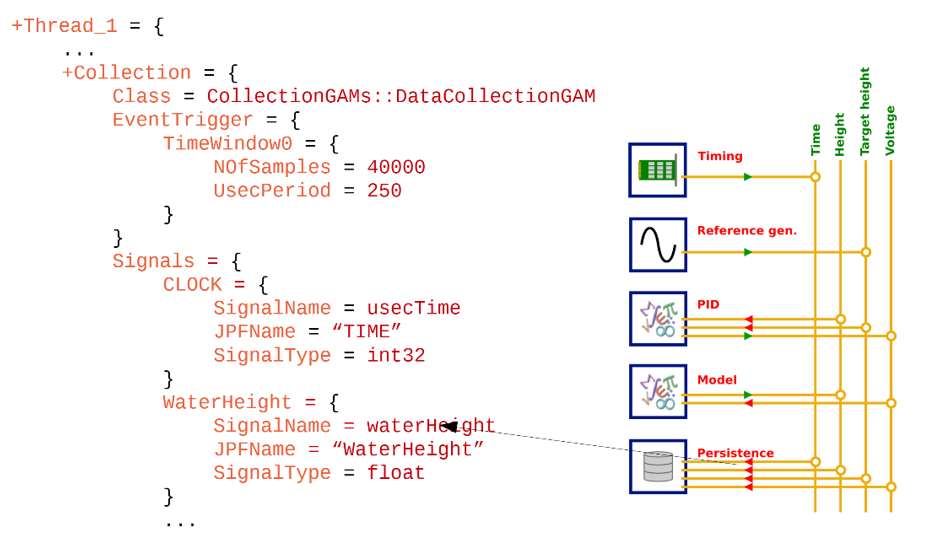
\includegraphics[width=1.0\textwidth]{MARTE.PNG}
\else
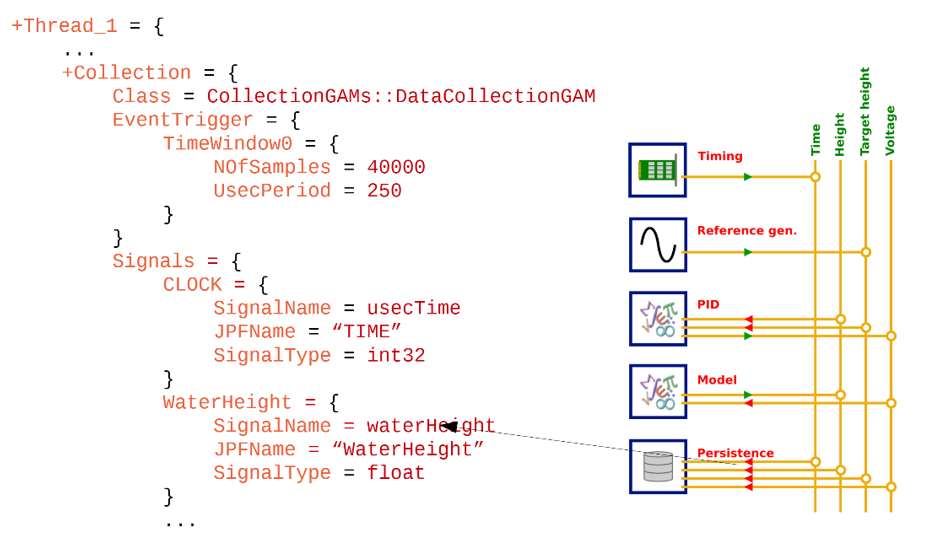
\includegraphics[width=0.5\textwidth]{MARTE.PNG}
\fi
\caption{The MARTe C++ real-time framework permits rapid composition of a new application
	from a deployment file which describes the component instances, attributes and links.
	Each application is a tree of cooperating objects.  The components have been designed
	to be compatible with robust, reliable, deterministic operation.}
\label{fig:MARTe}
\end{figure}

Fully proven on JET, for both control and protection applications
this would meet REQ-1 and REQ-3. Indeed, it was possible to select 
the latest release of the framework, MARTe2.  This has been 
developed under the management of F4E to provide integration for
a number of ITER systems. It includes some behavioural upgrades
which make development more efficient, and has been industrially
hardened\cite{netoAgileQualityAssurance2016}.  

A further beneficial feature arose from the JET real-time
network update in 2016\cite{waterhouseIntroductionITERCODAC2020a} to add support for the ITER 
Synchronous Databus Network (SDN). This made MARTe2
directly compatible with the available real-time signals.

Two alternative methods for porting the RTCC network calculation system 
to MARTe2 were considered. A monolithic approach, to wrap the calculation
engine from the heart of RTCC as a single MARTe2 component would have
had the least complexity in terms of testing.  However, this approach
would have provided no benefit in terms of evolving the system. 
Instead, each of the function blocks provided for RTCC were
individually ported as MARTe2 function components.  The benefit
of this scheme was that to extend the capability would only
need additional MARTe2 functions to be added, and this was a simple task.

The implementation therefore consisted of four tasks.  To create the 
MARTe2 application outline.  To port and test each of the 40 function
blocks.  To create a translation script to convert RTCC network
descriptions into MARTe2 format. To run integration tests based on
historical JET data to verify backwards compatibility.

\section{From Validation to Operation}
\label{s_validation}

As the software engineering work progressed, each of the deliverables
was progressively integrated with operations systems.  Wherever
possible, full coverage unit and integration tests were defined
in the UKAEA gitlab continuous integration (CI) system.
This included extensive regression tests of the integrated 
application against recorded data.  This tested not only
the correctness of the results, but the real-time performance.
  To achieve this required
some innovation in the use of containers as well as the
Yocto environment for building custom linux distributions.
%This is reported elsewhere by \cite{EdJones}.

JET machine management rules require strict adherence to procedures
for defining and executing commissioning procedures for critical 
systems\cite{kayeOperationJETUser2003}.  These procedures document the risks that have been 
identified for each system, the supporting mitigations that 
have been carried out prior to deployment, and the 
integrated online end to end checks which must be demonstrated
before a system can be used in full JET operation.

Figure~\ref{fig:vandv} lists the types of checks which were applied
to each of the software components. Consistent communication was primarily
assured by construction augmented by static code review and dynamic
validation of embedded metadata. 
RTCC2 configurations were also statically assured by
construction, with an extensive regression test suite to validate the 
code generation.
The python supervisor application consisted mostly of high-level
semantics with limited variability.  Manual code review of the
application and the deployment yaml files provided sufficient 
confidence in correctness.
Dynamic validation was finally achieved through the MARTe2 configuration 
parser proving application consistency at run-time.
Integrated validation was demonstrated during commissioning
where open circuit testing proved time-series equivalence.

\ifpreprint
\begin{figure}[p]
\else
\begin{figure}[ht!]
\fi
\centering
\ifpreprint
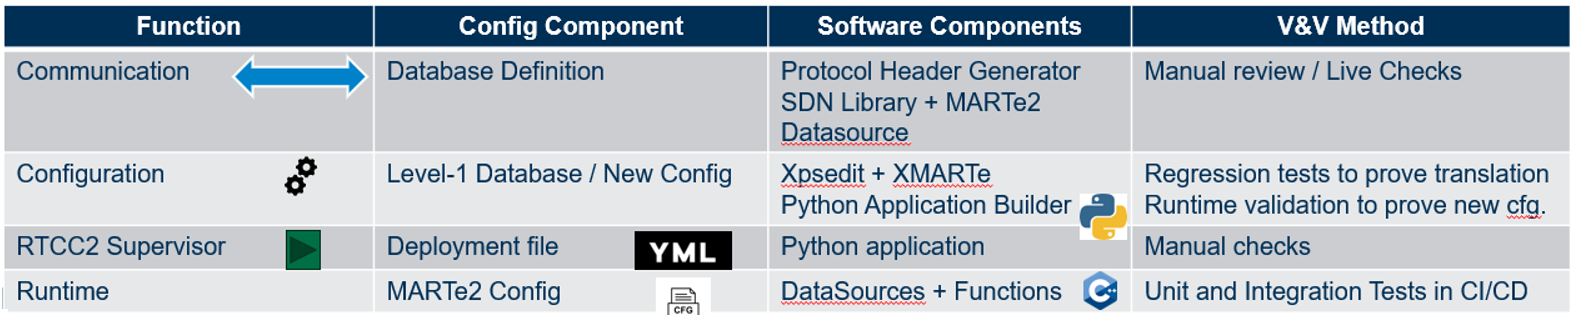
\includegraphics[width=1.0\textwidth]{VandV.png}
\else
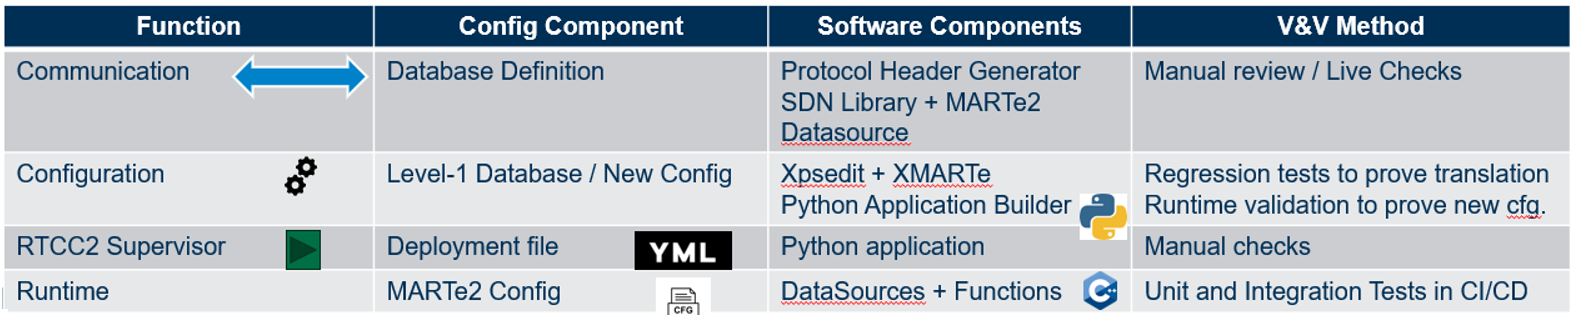
\includegraphics[width=0.5\textwidth]{VandV.png}
\fi
\caption{Validation and verification applied to each of the engineering categories related to delivering the upgrade.}
\label{fig:vandv}
\end{figure}


\subsection{Deployment - Modes of Operation}

JET operations had entered a particularly sensitive period at the time
when RTCC2 was ready for deployment. To further minimise the risk, 
senior management requested that the deployment plan allow for three
modes of operation
as shown in figure~\ref{fig:r1r2}.

The first mode was to retain the possibility to operate the full
control system with RTCC2 in parasitic mode. RTCC2 would carry
out all of the normal operations, would run connected to the
real-time network, but {\em only} as a passive consumer.
This eliminated almost all risk and was appropriate for any
experiment which only needed RTCC1 capability.
This mode was also an opportunity to exercise RTCC2 in the
production environment and prove readiness for use.

The second mode would permit RTCC2 to send control requests
arising from executing control networks, but only to RTCC1.
RTCC1 would then be able to select from the RTCC2 results
to directly control the actuator systems.  This opened 
up the extended capacity and capability of RTCC2, but 
eliminated any possibility of unexpected interactions 
between RTCC2 and the actuator systems, at the cost of
one extra timestep delay.

The third mode would enable full RTCC2 operation, to
execute control networks, and to directly control the
actuator systems.

\ifpreprint
\begin{figure}[p]
\else
\begin{figure}[ht!]
\fi
\centering
\ifpreprint
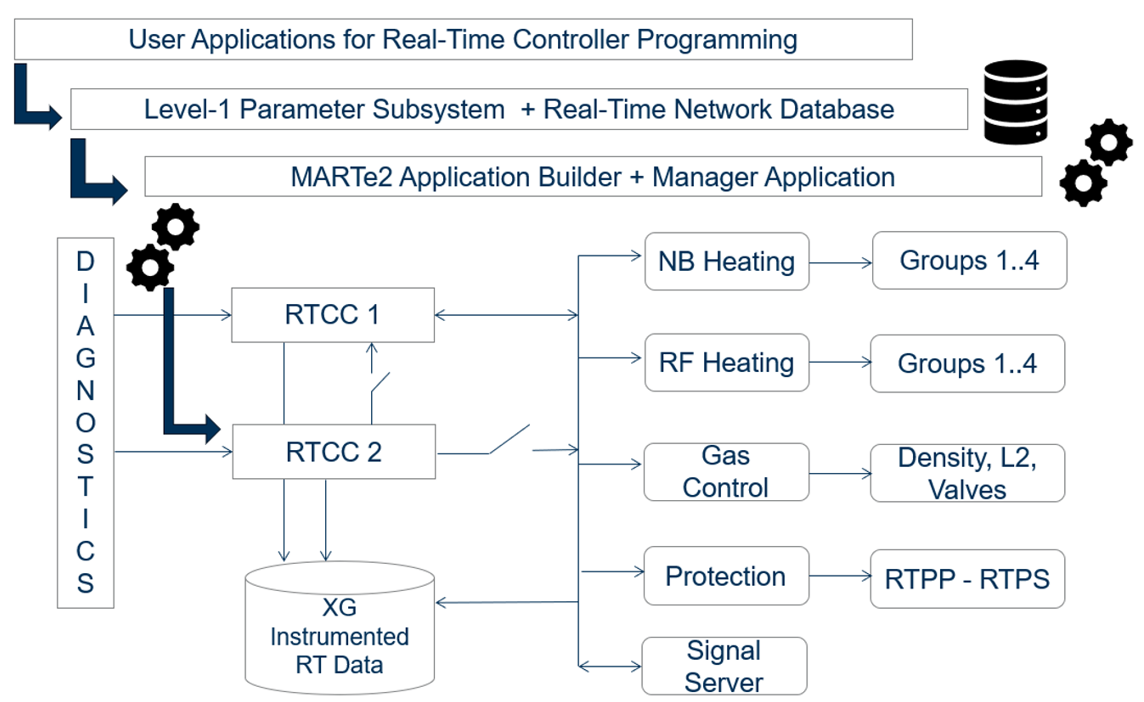
\includegraphics[width=1.0\textwidth]{R1R2ARCH.PNG}
\else
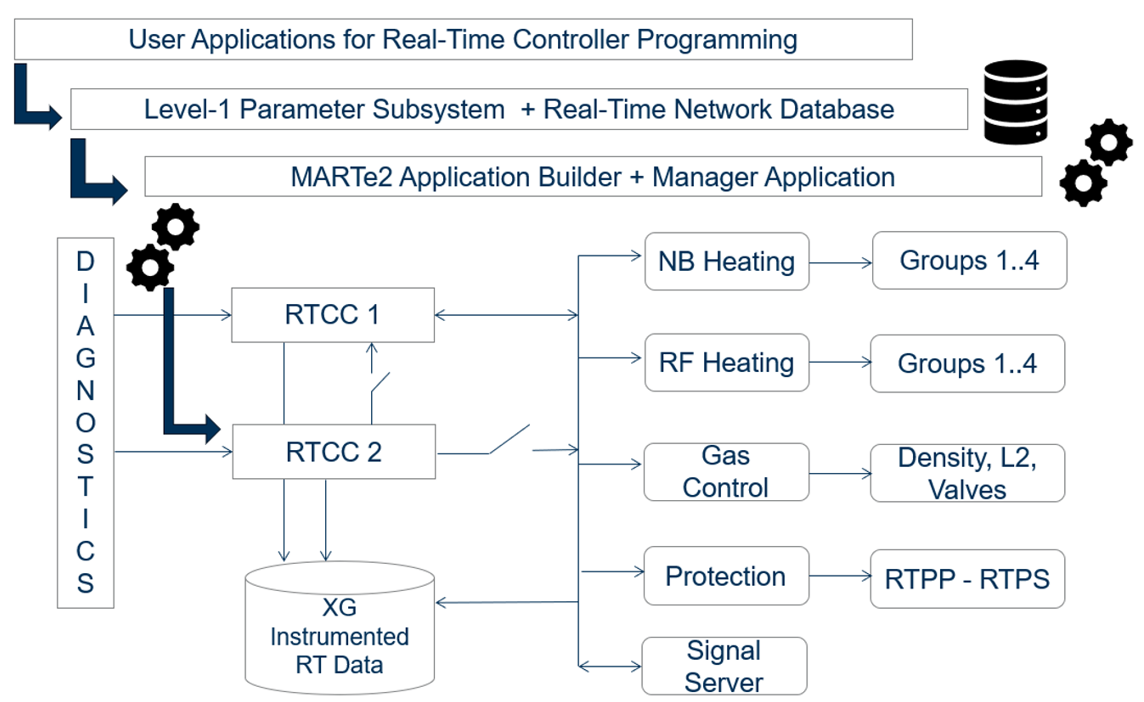
\includegraphics[width=0.5\textwidth]{R1R2ARCH.PNG}
\fi
\caption{Multiple modes of operation were requested to reduce
the risk of updating the plasma control system at a particularly
	sensitive time for JET operations.}
\label{fig:r1r2}
\end{figure}

\subsection{Outcomes}

All of the engineering to develop the new RTCC2 system were completed.
In addition to the new MARTe2 components and the tooling for automatic
conversion of RTCC control schemes to MARTe2 format, a graphical
user interface was created.  This provides a more intuitive way to both
view, and edit, these control graphs.

The extensive quality assurance evidence (described in \S~\ref{s_validation})
was sufficient to 
justify a commissioning procedure which had a minimal requirement
for machine time to verify system conformity.  This is an important
point as machine time is very expensive.

The new system entered parasitic testing from JPN 101487.  The upgraded
functionality was communicated to the task force experiment teams in 
January 2023.  New components were requested to support implementation
of an X-point radiation tracker control. The benefits of MARTe2 as
an effective environment in which to develop new modules was proven
as vector processing and a peak detector components were quickly added.
The vector processing significantly reduced the complexity of 
the networks.  These features were used to succcessfully support detachment
control experiments.


\section{Discussion}

It is useful to analyse the architecture of the RTCC2 solution
in the context of modern trends in systems design.

Top-down design approaches look to start from formal requirements.
High-level designs are then developed using Model-Based Systems
Engineering (MBSE). Models are represented in formal modelling
languages. Computer aided tools for MBSE support textual and
graphical descriptions.  Formerly limited to static documents,
the current generation of applications can include quantitative,
executable simulations.  The focus is on modelling the system
domain, independent of implementation issues. 

JET predated the rise of model based design tools.  However, the
core parameter management system (Level-1) can be seen as a system
which captures the main domain concepts and relationships. It provides
the interfaces within which the science and engineering experts
encode the target behaviour to be delivered by the control system.

ITER is more directly applying modern methods and the PCS
design is developed using formal Systems Engineering.
These models document the control models which are
developed in Matlab/Simulink so that they can be
quantitatively be demonstrated to work correctly.

Turning to the implementation side, software engineers must
design a framework suitable to achieve the goals of the models.
Design models in UML are typically produced along with the software.
In some contexts, this is similar to the systems engineering.
More typically though, the lead architects will seek to 
leverage abstraction to achieve a modular design of components.
This methodology may value reusability across projects
above ruthless traceability to requirements.

JET software frameworks in general have had a strong tradition
of reusability, initially using data-driven patterns.  The
original RTCC system is a good example of this.  As JET became
increasingly complex, it was recognised that factoring out
the recurring engineering costs common to classes of application
was essential. This resulted in the MARTe concept which 
strongly decouples reusable code from modifiable configuration.

ITER has followed this pattern. It has adopted and enhanced
the original JET framework, now MARTe2. It has also commissioned
an independent Real-Time Framework (RTF) specifically for the core plasma
control system. The provision of dual redundant software 
systems gives advantages in terms of resilience for the protection system.

Both domain and implementation designers seek to deal with the complexity of large
systems through phases of analysis to deconstruct 
followed by sythensis to compose. Each seeks to balance 
investment in flexible elements which yield resilience
against scope creep which may add cost and risk.

Traditional approaches to bring the domain design and implementation
into alignment rely on teams of experts iterating manually.
As with other fusion design problems, the limitation of this
approach is that early assumptions tend to make the 
dependencies between the two worlds fragile.
The additional cost of adding a late change to the 
high level model can be severe for the implementation team.
Conversely, ensuring that modest changes in the implementation
find adequate representation and traceability in the system
engineering can also be challenging.
Maintaining design integrity across both domains efficiently
demands a holistic approach.

One route is to use modelling tools which incorporate code
generation capability.  This is starting to become possible,
and indeed the ITER approach expects to do exactly this.
The technique is not without risk, since the challenge is
not simply to generate production code that directly
reproduces the control models.  Practical aspects like 
operating system interfaces, data acquisition drivers,
timing and hardware constraint management must be considered.

A variation on the theme is neatly encapsulated by the example
of RTCC/RTCC2 and underpins the design goals of MARTe. 
This is to use the modelling tool to perform code generation,
but with a domain specific target language.  
For the RTCC application, this target language described 
the control algorithms in terms of abstract operators 
(the function blocks), real-time plasma signals as inputs,
and parameters values (gains, coefficients).
It was this abstraction that enabled a simple and low risk
approach to migrating the application to a new software framework.
By maintaining the conceptual interface between the physics
operators and the run-time engine, it was possible to have
high confidence that the replacement system would deliver
equivalent functionality.  The additional testing to 
prove the confidence was warranted because of the financial
and project risks, but it was important in order to 
approve the project from the outset.

When debating design approaches, it is recognised that
in theory, there is no difference
between high-level and low-level languages.  As long as they are
Turing complete they are functionally equivalent. 
In practice, the effectiveness of using different types
of language for different engineering workflows is
important.  As Feynman said, "Notation is powerful.  Invent it.".


\section{Conclusion}

% Comments on DSLs and tooling.
The RTCC system enabled JET real-time control experiments to adapt rapidly to new information
and ideas because the round trip time from concept to implementation did not require 
external software engineering. This was made possible by offering a flexible, but 
constrained programmable environment.

The project to upgrade RTCC 
successfully delivered the minimum project goals of increased capacity with
full backwards compatibility to reuse all previous control scheme definitions.
This was done without loss of operational time.
In addition, the stretch goals of increasing capability and improving
usability for end users were addressed.  

This change to a critical part of the JET plasma control system, implemented
at one of the most sensitive times in the programme life was enabled by 
sound historical architecture choices. These were both based on abstracting
the definition of real-time data flow and processing into machine 
processable formats. In respect of inter-system communication, this was the
real-time data network database, implemented using CODAS Configuration Language
(CCL) with automatic code generation.  In respect of intra-system algorithm
representation, this was via the RTCC network graph, and the equivalent RTCC2
object graph.  

The project feasibility rested not solely on these architectural patterns,
but on the MARTe framework and the improvements
and extensions made to this software in preparation for ITER.  
The JET real-time network extension to ethernet and use of SDN in 2016
provided a solid foundation.  The quality assurance and functional updates delivered
by the F4E MARTe2 project reduced the RTCC upgrade risk to an acceptable level.

JET innovations in control system architecture have proved their value 
in many contexts. The power of inventing effective programming tools
to cope with the growing complexity in modern systems is well recognised
in other fields.  It is hoped that this project will make the case for
continued investment in fusion control systems software. To quote the
motto of the Software Sustainability Institute, "Better Software, Better Research".

The JET real-time algorithm executor has been ported to a future-proof and future-relevant framework.
The implementation leaves the possibility to rerun former JET shots against a virtualised
version of RTCC2. This opens the possibility to running virtual JET experiments.
These can test alternative state estimation concepts just by replaying the historic data.
By replacing dynamic elements with models, a closed loop virtual JET emulator could be demonstrated.
This could have a number of valuable uses.




%%\section{Glossary}
%%
%%
%%Field specific terms.
%%\begin{itemize}
%%\item[ATM]{Asynchronous Transmission Mode.  A low-latency telecommunications protocol standard.}
%%\item[DSL]{Domain Specific Language}
%%\item[MARTe]{Multi-threaded Application for Real-Time execution.  Software framework from JET.}
%%\item[MARTe2]{Enhanced version of MARTe developed by F4E for ITER.}
%%\item[Real-Time Thread]{The unit of concurrency in a MARTe2 application.}
%%\item[DataSource]{A service which abstracts device drivers to handle application I/O in a MARTe2 application.}
%%\item[Function]{The unit of compute in a MARTe2 application.  Each Real-Time Thread calls one or more Functions.}
%%\item[JET]{Joint European Tokamak}
%%\item[MBSE]{Model Based System Engineering}
%%\item[PCS]{Plasma Control System}
%%\item[RTCC]{Real-Time Central Controller.  A core application in the JET PCS.}
%%\item[SDN]{Synchronous Databus Network.  An ITER real-time network protocol.}
%%\item[UDP]{User Datagram Protocol. A connectionless data transport method in networking.}
%%\end{itemize}

\section{Abbreviations}


\begin{description}
%\begin{itemize}
	\item[ATM] Asynchronous Transmission Mode
	\item[DSL] Domain Specific Language
	\item[MARTe] Multi-threaded Application for Real-Time execution
	\item[JET] Joint European Tokamak
	\item[MBSE] Model Based System Engineering
	\item[PCS] Plasma Control System
	\item[RTCC] Real-Time Central Controller
	\item[SDN] Synchronous Databus Network
	\item[UDP] User Datagram Protocol
%
		
	%\item{ATM}{Asynchronous Transmission Mode}
	%\item{DSL}{Domain Specific Language}
	%\item{MARTe}{Multi-threaded Application for Real-Time execution}
	%\item{JET}{Joint European Tokamak}
	%\item{MBSE}{Model Based System Engineering}
	%\item{PCS}{Plasma Control System}
	%\item{RTCC}{Real-Time Central Controller}
	%\item{SDN}{Synchronous Databus Network}
	%\item{UDP}{User Datagram Protocol}
%\end{itemize}
\end{description}

\section{Acknowledgements}

The MARTe software has been developed over a long time by members of the fusion community.
Much of the software engineering that delivered the RTCC system and many other
JET real-time systems was the work of Quentin King.

\section{Funding}
JET, which was previously a European facility, is now a UK facility collectively used by all European fusion laboratories under the EUROfusion consortium.  It is operated by the United Kingdom Atomic Energy Authority, supported by DESNZ and its European partners. This work, which has been carried out within the framework of the Contract for the Operation of the JET Facilities up to 31 October 2021, has been funded by the Euratom Research and Training  Programme.  Since 31 October 2021, UKAEA has continued to work with the EUROfusion Consortium as an Associated Partner of Max-Plank-Gesellschaft zur Förderung der Wissenschaft e.V represented by Max-Plank-Institut fur Plasmaphysik (“IPP”) pursuant to Article 9.1 of the EUROfusion Grant Agreement for Project No 101052200.   The views and opinions expressed herein do not necessarily reflect those of the European Commission.

\bibliographystyle{elsarticle-num}
\bibliography{IAEA24}{}

\end{document}

%\endinput
